\documentclass{article}

\usepackage{url}
\usepackage{alltt}
\usepackage{upquote}
\usepackage{xspace}
\usepackage[usenames,dvipsnames]{color}
\usepackage{graphicx}
\usepackage{float}

\newcommand{\inp}[1]{\texttt{\underline{#1}}}
\newcommand{\txt}[1]{\texttt{#1}}
\newcommand{\promptm}{wcaarls@vbox:\~{}/src/grl\$\xspace}
\newcommand{\promptmb}{wcaarls@vbox:\~{}/src/grl/build\$\xspace}
\newcommand{\promptmn}{wcaarls@vbox:\~{}/src/grl/bin\$\xspace}

\newcommand{\prompt}{wcaarls@vbox:\~{}\$\xspace}
\newcommand{\prompth}{wcaarls@vbox:\~{}/indigo\_ws\$\xspace}
\newcommand{\prompths}{wcaarls@vbox:\~{}/indigo\_ws/src\$\xspace}

\newenvironment{code}{\alltt}{\endalltt}

\title{GRL: a generic C++ reinforcement learning library}
\author{Wouter Caarls $<$\url{mailto:wouter@caarls.org}$>$}
\date{October 5th, 2015}
\begin{document}
\maketitle

\section{Introduction}

GRL is a C++ reinforcement learning library that aims to easily allow
evaluating different algorithms through a declarative configuration
interface.

\section{Directory structure}

\begin{verbatim}
.
|-- base                     Base library
|   |-- include              Header files
|   `-- src                  Source files
|       |-- agents           Agents (fixed, black box, td)
|       |-- discretizers     Action discretizers
|       |-- environments     Environments (pendulum, cart-pole)
|       |-- experiments      Experiments (online, batch)
|       |-- policies         Control policies (PID, Q-based)
|       |-- predictors       Value function predictors (SARSA, AC)
|       |-- projectors       State projectors (tile coding, fourier)
|       |-- representations  Representations (linear, ann) 
|       |-- samplers         Action samplers (greedy, e-greedy)
|       |-- solvers          MDP solvers (VI, rollout-based)
|       |-- traces           Elibility traces (accumulating, replacing)
|       `-- visualizations   Visualizations (value function, policy)
|-- addons                   Optional modules
|   |-- cma                  CMA-ES black-box optimizer
|   |-- gl                   OpenGL-based visualizations
|   |-- glut                 GLUT-based visualizer
|   |-- llr                  Locally linear regression representation
|   |-- lqr                  Linear Quadratic Regulator solver
|   |-- matlab               Matlab interoperability
|   |-- muscod               Muscod interoperability
|   |-- odesim               Open Dynamics Engine environment
|   |-- rbdl                 Rigid Body Dynamics Library dynamics
|   `-- ros                  ROS interoperability
|-- bin                      Python binaries (configurator)
|-- externals                Imported external library code
|-- cfg                      Sample configurations
|-- share                    Misc files
|   `-- taskmaster           Taskmaster parameter study example
|-- tests                    Unit tests
|-- CMakeLists.txt           CMake instructions to build everything
`-- grl.cmake                CMake helper functions
\end{verbatim}

\section{Prerequisites}

GRL requires some libraries in order to compile. Which ones exactly depends
on which agents and environments you would like to build, but the full list
is

\begin{itemize}
  \item Git
  \item GCC (including g++)
  \item Eigen
  \item GLUT
  \item ZLIB
  \item QT4 (including the OpenGL bindings)
  \item TinyXML
  \item MuParser
  \item ODE, the Open Dynamics Engine
  \item Python (including Tkinter and the yaml reader)
  \item Lua
\end{itemize}

On Ubuntu 16.04, these may be installed with the following command:

\begin{code}
\prompt \inp{git cmake g++ libeigen3-dev \textbackslash}
\inp{libgl1-mesa-dev freeglut3-dev libz-dev libqt4-opengl-dev \textbackslash}
\inp{libtinyxml-dev libmuparser-dev libode-dev python-yaml python-tk \textbackslash}
\inp{liblua5.1-dev}
\end{code}

\section{Building}

GRL may be built with or without ROS's catkin. When building with, simply
merge \txt{grl.rosinstall} with your catkin workspace

\begin{code}
{\color{Gray}\prompt \inp{mkdir indigo\_ws}
\prompt \inp{cd indigo\_ws}
\prompth \inp{rosws init src /opt/ros/indigo}
\prompth \inp{cd src}}
\prompths \inp{rosws merge /path/to/grl.rosinstall} 
\prompths \inp{rosws up}
\prompths \inp{cd ..}
\prompth \inp{catkin\_make}
\end{code}

Otherwise, follow the standard CMake steps of (in the \txt{grl} directory)
\begin{code}
\promptm \inp{mkdir build}
\promptm \inp{cd build}
\promptmb \inp{cmake ..}
\txt{-- The C compiler identification is GNU 4.8.2}
\txt{...}
\promptmb \inp{make}
\txt{Scanning dependencies of target yaml-cpp}
\txt{...}
\end{code}

\section{Running}

The most important executables in grl are the deployer (\txt{grld}) and
configurator (\txt{grlc}). The configurator allows you to generate configuration
files easily. To see an example, run

\begin{code}
\promptmn ./grlc ../cfg/pendulum/sarsa\_tc.yaml
\end{code}

More information on the configurator can be found in
Section~\ref{sec:grlc}. Once you have configured your experiment, you can either run it directly
from the configurator, or save it and run it using the deployer. For
example:

\begin{code}
\promptmb ./grld ../cfg/pendulum/sarsa\_tc.yaml
\end{code}

\section{Build environment}

The whole \txt{grl} system is built as a single package, with the exception
of \txt{mprl\_msgs}. This is done to facilitate building inside and outside
catkin. There is one \txt{CMakeLists.txt} that is used in both cases. The
ROS interoperability is selectively built based on whether \txt{cmake} was invoked by
\txt{catkin\_make} or not.

Modules are built by calling their respective \txt{build.cmake} scripts,
which is done by \txt{grl\_build\_library}. The include directory is set
automatically, as is an \txt{SRC} variable pointing to the library's source
directory.

The build system has a simplistic dependency management scheme through
\txt{grl\_link\_libraries}. This calls the \txt{link.cmake} files of the
libraries on which the current library depends. Typically they will add some
\txt{target\_link\_libraries} and add upstream dependencies.
\txt{grl\_link\_libraries} also automatically adds the upstream library's
include directory.

\section{Class structure}

Most classes in grl derive from \txt{Configurable}, a base class that
standardizes configuration such that the object hierarchy may be constructed
declaratively in a configuration file. Directly beneath \txt{Configurable}
are the abstract base classes defining the operation of various parts of the
reinforcement learning environment, being:
\begin{description}
\item[\txt{Agent}] RL-GLUE\footnote{\url{http://http://glue.rl-community.org}}
style agent interface, receiving observations in an episodic manner and returning
actions.
\item[\txt{Discretizer}] Provides a list of discrete points spanning a
continuous space.
\item[\txt{Environment}] RL-GLUE style environment interface, receiving
actions and returning observations.
\item[\txt{Experiment}] Top-level interface, which typically calls the agent
and environment in the correct manner, but may in general implement any
experiment.
\item[\txt{Optimizer}] Black-box optimization of control policies,
suggesting policies and acting on their cumulative reward.
\item[\txt{Policy}] Basic control policy that implements the state-action
mapping.
\item[\txt{Predictor}] Basic reinforcement learning interface that uses
transitions to predict a value function or model.
\item[\txt{Projector}] Projects an observation onto a feature vector,
represented as a \txt{Projection}.
\item[\txt{Representation}] Basic supervised learning interface that uses
samples to approximate a function. As such, it generally supports reading,
writing and updating of any vector-to-vector mapping.
\item[\txt{Sampler}] (Stochastically) chooses an item from a vector of (generally
unnormalized) values.
\item[\txt{Trace}] Stores a trace of projections with associated
eligibilities that can be iterated over.
\item[\txt{Visualization}] Draws on the screen to visualize some aspect of
the learning process.
\item[\txt{Visualizer}] Keeps track of visualizations and provides the
interface to the graphics subsystem.
\end{description}

Each abstract base class is generally implemented in various concrete
classes, with or without additional hierarchy. A list can be requested by
running 

\begin{code}
\promptmn ./grlq
\end{code}

and is also available in the appendices of this document.

A typical example of the information flow between the various classes can be seen in Figure~\ref{fig:td},
which depicts the standard TD control setting.

\begin{figure}
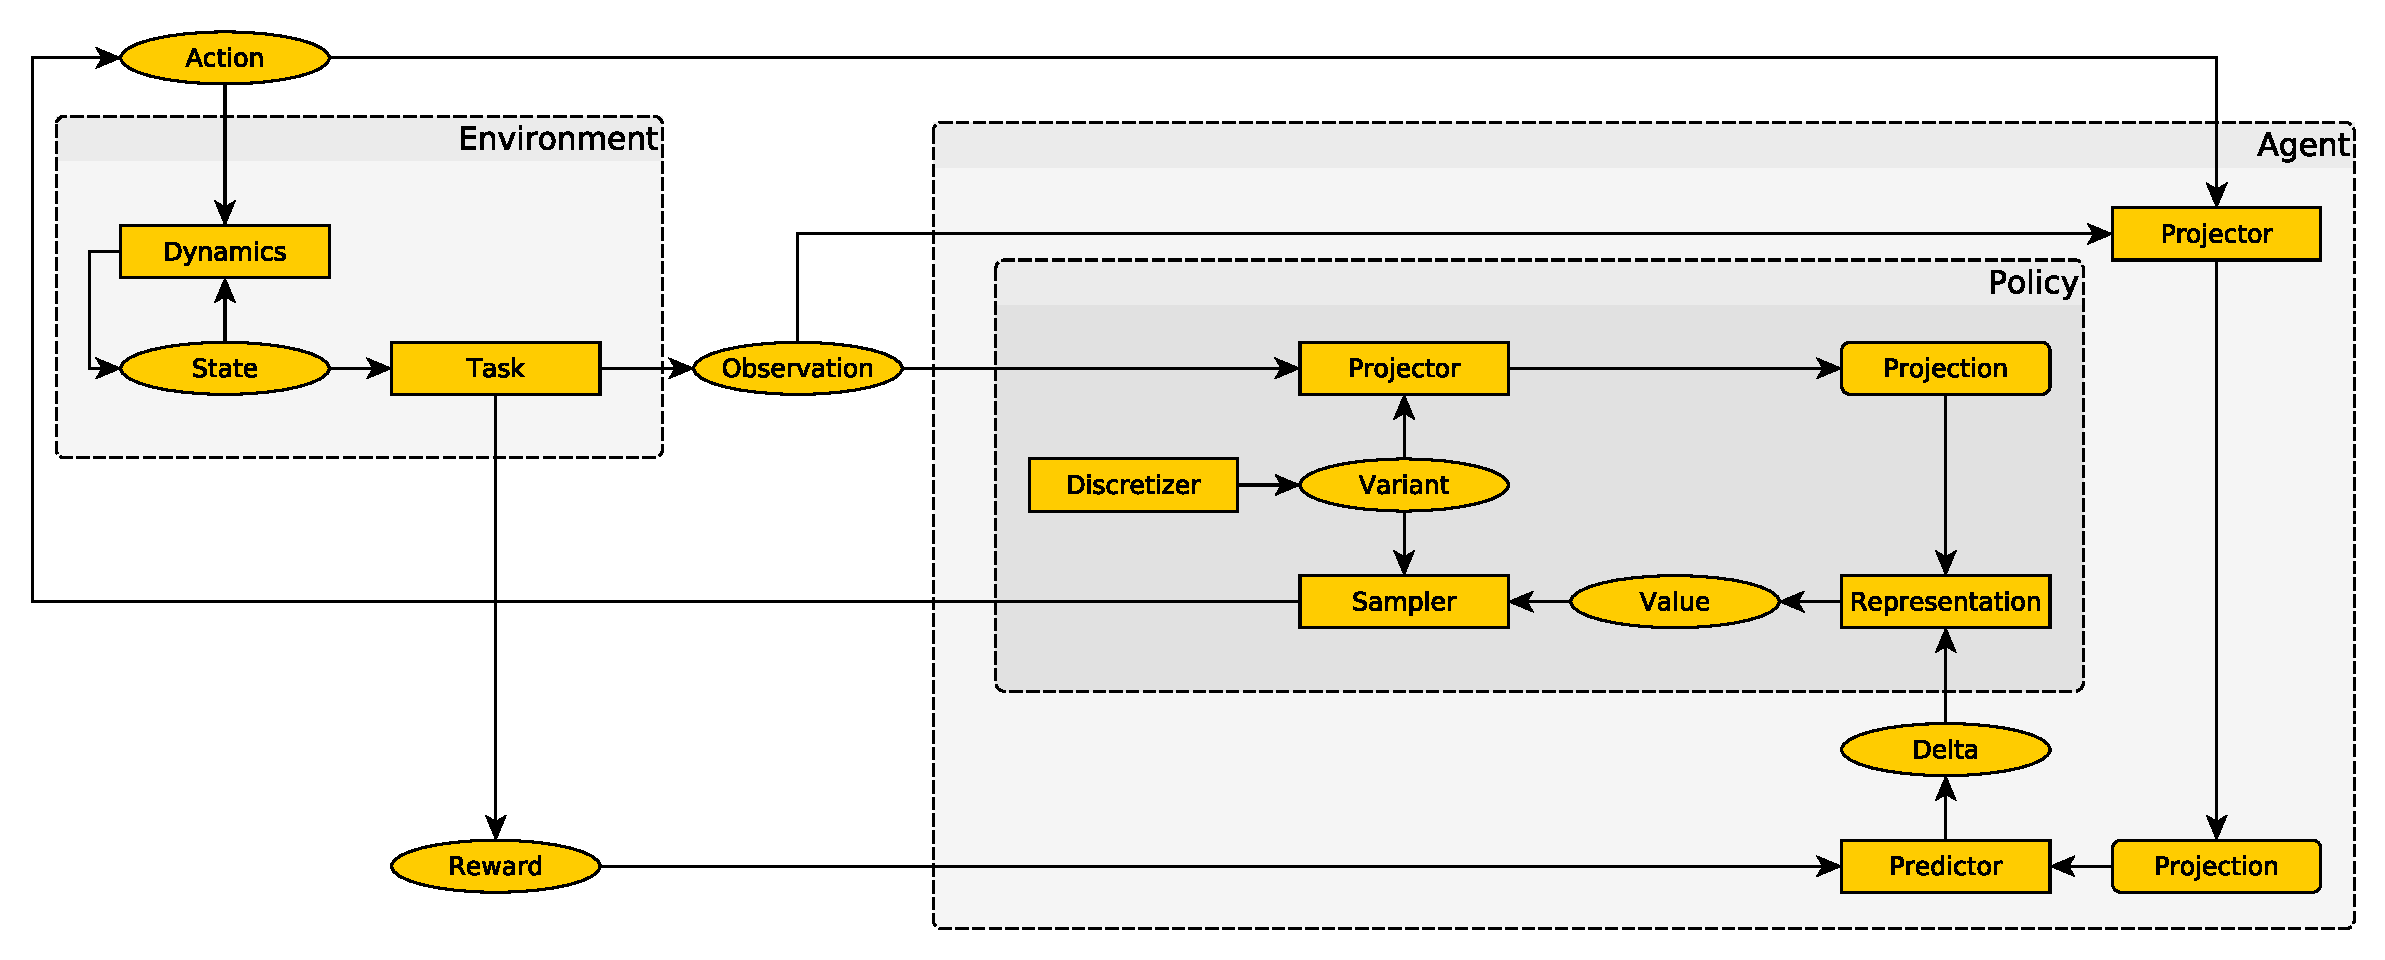
\includegraphics[width=\linewidth]{td.pdf}
\caption{Information flow diagram for regular TD control. Rectangles (and
dashed rectangles) are \txt{Configurable} objects, while the others are the
data passed between them.}
\label{fig:td}
\end{figure}

\subsection{Configuration}

Each \txt{Configurable} subclass must define its type and a short
description using the \txt{TYPEINFO} macro:

\begin{code}
class OnlineLearningExperiment : public Experiment
\{
  public:
    TYPEINFO("experiment/online_learning", "Interactive learning experiment")
  
  /* ... */
\};
\end{code}

This textual description of the type is used to facilitate user
configuration by limiting the selection of parameter values, as well as enforcing the type
hierarchy. In general, the textual description should follow the C++ class
hierarchy, but this is not obligatory.

The basic \txt{Configurable} interface has three important functions:

\subsubsection{\txt{request}}
\begin{code}
virtual void request(ConfigurationRequest *config);
\end{code}

\txt{request} is called by the configurator to find out which parameters the
object requires to be set, and which parameters it exports for other objects
to use. To do this, it should extend the given \txt{ConfigurationRequest}
by pushing configuration request parameters (\txt{CRP}s). A basic \txt{CRP}
has the following signature:

\begin{code}
CRP(string name, string desc, TYPE value)
\end{code}

where TYPE is one of int, double, Vector, or string. For example:

\begin{code}
config->push_back(CRP("steps", "Number of steps per learning run", steps_));
config->push_back(CRP("output", "Output base filename", output_));
\end{code}

The \txt{value} argument is used both to determine the type of the parameter
and the default value suggested by the configurator. \txt{request} may also
be called while the program is running, in which case it is expected to
return the current value of all parameters.

To use other \txt{Configurable} objects as parameters, use

\begin{code}
CRP(string name, string type, string desc, Configurable *value)
\end{code}

The extra \txt{type} field restricts which \txt{Configurable} objects may
be used to configure this parameter. Only objects whose \txt{TYPEINFO}
starts with the given \txt{type} are eligible. For example:

\begin{code}
config->push_back(CRP("policy", "policy/parameterized",\\
                      "Control policy prototype", policy_));
\end{code}

restricts the \txt{"policy"} parameter to classes derived from
\txt{ParameterizedPolicy}. Note that this extra type hierarchy is related
to, but not derived from the actual class hierarchy. Care must therefore be
taken in the correct usage of \txt{TYPEINFO}.

Some parameters are not requested, but rather \emph{provided} by an object. In
that case. These have the following signature:

\begin{code}
CRP(string name, string type, string desc, CRP::Provided)
\end{code}

Examples of provided parameters are the number of observation dimensions
(provided by \txt{Task}s) or the current system state (provided by some
\txt{Environment}s).

\subsubsection{\txt{configure}}

\begin{code}
virtual void configure(Configuration *config);
\end{code}

\txt{configure} is called after all parameters (including other
\txt{Configurable} objects) have been initialized. The parameter values may
be accessed using mapping syntax (\txt{config["parameter"]}). Note that
\txt{Configurable} objects are passed as void pointers and must still be cast to
their actual class:

\begin{code}
steps_ = config["steps"];  
output_ = config["output"].str();
policy_ = (ParameterizedPolicy*)config["policy"].ptr();
\end{code}

Note the use of \txt{.str()} and \txt{.ptr()} for strings and objects,
respectively. Provided parameters should be written to the configuration
instead of read, like so:

\begin{code}
config.set("state", state_);
\end{code}

\subsubsection{\txt{reconfigure}}
\begin{code}
virtual void reconfigure(const Configuration *config);
\end{code}

Some parameters may be defined as reconfigurable by appending
\txt{CRP::Online} to the respective \txt{CRP} signature. In the case of a
reconfiguration, \txt{reconfigure} will be called with the new values of
those parameters in \txt{config}. \txt{reconfigure} may also be used for
general messaging, equivalent to RL-GLUE's \txt{message} calls. In that
case, it is often helpful to reconfigure all objects in the object
hierarchy, which can be done using

\begin{code}
void Configurable::walk(const Configuration &config);
\end{code}

Examples are resetting the hierarchy for a new run (\txt{config["action"] =
"reset"}) or saving the current state of all memories (\txt{config["action"]
= "save"}). In the latter case, \txt{Configurable::path()} may be used to
determine an object's location in the object hierarchy.

\subsection{Roles}

While using the configurator, the user often has to select previously
defined objects as the value of certain parameters. If all such previously
defined objects are presented as possibilities, the list would quickly grow
very large. To make setting these parameters easier, a class may have
various \emph{roles} while providing the same interface. In that case,
only previously defined objects with a role that starts with the requested
role are valid choices.

An example is a \txt{Representation}, which may represent a state-value function,
action-value function, control policy or model. Each has a different number
of inputs and outputs, and chosing the wrong representation will result in
mismatches. An object requesting a \txt{Representation} may therefore request
a certain role. For example:

\begin{code}
config->push_back(CRP("representation", "representation.value/action",\\
                      "Q-value representation", representation_));
\end{code}

requests any representation that represents action-values. A newly
defined \txt{representation} will do, of course, but from the previously
defined ones only the ones with the right role are eligible.

The same strategy is used for basic types, for example:

\begin{code}
config->push_back(CRP("outputs", "int.action_dims",
                      "Number of outputs", outputs_, CRP::System));
\end{code}

make sure the only suggested previously defined values for the
\txt{"outputs"} parameter are ones with the \txt{"action\_dims"} role. As an added
convenience, if the parameter is defined as a \emph{system parameter}
(\txt{CRP::System}), meaning that the choice is not free but rather defined
by the structure of the configuration, and only a single value was
previously defined, that value is automatically used.

The role that needs to be requested may depend on the role of the requesting
object itself. In that case, the following signature for \txt{request}
should be used:

\begin{code}
virtual void request(const std::string \&role, ConfigurationRequest *config);
\end{code}

\section{Configurator}
\label{sec:grlc}

\begin{figure}[H]
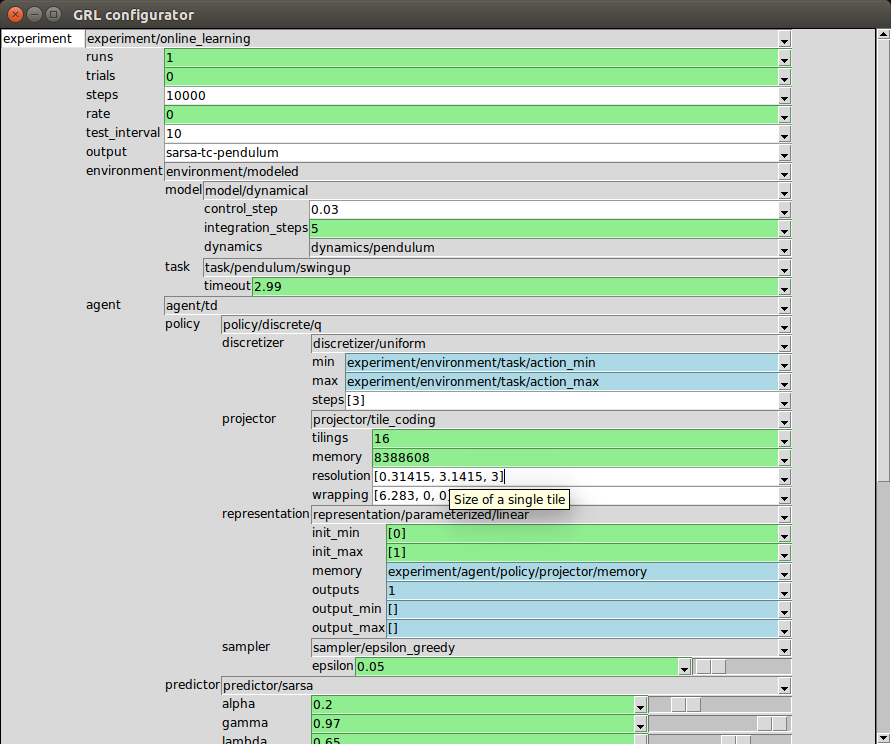
\includegraphics[width=\linewidth]{grl.png}
\caption{Python configurator user interface}
\label{fig:conf}
\end{figure}

\section{Matlab interface}

If Matlab is installed (and can be found on the path), a MEX interfaces for
the agents and environments is built. If you want to use these, make sure
that you're building with a compatible compiler, both by setting the
\txt{CC} and \txt{CXX} variables in your call to \txt{cmake} and by correctly
configuring \txt{mex}.

\subsection{Environments}

To initialize an environment, call

\begin{code}
>> spec = grl_env('cfg/matlab/pendulum_swingup.yaml');
\end{code}

Where the argument specifies a configuration file that has a top-level
'environment' tag. \txt{spec} gives some information about the environment,
such as number of dimensions, minimum and maximum values, etc. Next,
retrieve the first observation of an episode with

\begin{code}
>> o = grl_env('start');
\end{code}

where \txt{o} is the observation from the environment. All following
steps should be called using

\begin{code}
>> [o, r, t, d] = grl_env('step', a);
\end{code}

where \txt{a} is the action suggested by the agent, \txt{r} is the reward
given by the environment, \txt{t} signals termination of the episode and 
txt{d} is the length of the step.
If \txt{t} is 2, the episode ended in an absorbing state. When all episodes
are done, exit cleanly with

\begin{code}
>> grl_env('fini');
\end{code}

\subsection{Agents}

To initialize the agent, use

\begin{code}
>> grl_agent('init', 'cfg/matlab/sarsa.yaml');
\end{code}

Where the argument specifies a configuration file that has a top-level
'agent' tag. Next, give the first observation of an episode with

\begin{code}
>> a = grl_agent('start', o);
\end{code}

where \txt{o} is the observation from the environment and \txt{a} is the
action suggested by the agent. All following steps should be called using

\begin{code}
>> a = grl_agent('step', d, r, o);
\end{code}

where \txt{r} is the reward given by the environment and 
txt{d} is the length of the step. To signal the end of
an episode (absorbing state), use

\begin{code}
>> a = grl_agent('end', d, r);
\end{code}

To end an episode without an absorbing state, simply start a new one. To
exit cleanly after all epsiodes are finished (which also allows you to
reinitialize the agent with different options), call

\begin{code}
>> grl_agent('fini');
\end{code}

\appendix

\section{Agents}
\subsection{agent/black\_box}
\noindent Agent that learns from the cumulative reward of complete rollouts\\

\noindent\begin{tabular}{@{}lll@{}}
episodes&int&Number of episodes to evaluate policy\\
optimizer&optimizer&Policy optimizer\\
\end{tabular}
\subsection{agent/dyna}
\noindent Agent that learns from both observed and predicted state transitions\\

\noindent\begin{tabular}{@{}lll@{}}
planning\_steps&int&Number of planning steps per control step\\
planning\_horizon&int&Planning episode length\\
asynchronous&int&Asynchronous planning (actual planning\_steps depends on control step time and processing power)\\
policy&policy&Control policy\\
predictor&predictor&Value function predictor\\
model&observation\_model&Observation model used for planning\\
model\_predictor&predictor/model&Model predictor\\
model\_agent&agent&Agent used for planning episodes\\
\end{tabular}
\\

\noindent Provided parameters\\

\noindent\begin{tabular}{@{}lll@{}}
state&state&Current observed state of planning\\
\end{tabular}
\subsection{agent/fixed}
\noindent Fixed-policy agent\\

\noindent\begin{tabular}{@{}lll@{}}
policy&policy&Control policy\\
\end{tabular}
\subsection{agent/master/exclusive}
\noindent Master agent that selects one sub-agent to execute\\

\noindent\begin{tabular}{@{}lll@{}}
gamma&double&Discount rate\\
agent1&agent/sub&First subagent\\
agent2&agent/sub&Second subagent\\
\end{tabular}
\subsection{agent/master/sequential}
\noindent Master agent that executes sub-agents sequentially\\

\noindent\begin{tabular}{@{}lll@{}}
agent1&agent&First subagent, providing the suggested action\\
agent2&agent&Second subagent, providing the final action\\
\end{tabular}
\subsection{agent/solver}
\noindent Agent that successively solves learned models of the environment\\

\noindent\begin{tabular}{@{}lll@{}}
interval&int&Episodes between successive solutions (0=asynchronous)\\
policy&policy&Control policy\\
predictor&predictor&Optional (model) predictor\\
solver&solver&Model-based solver\\
\end{tabular}
\subsection{agent/sub/compartmentalized}
\noindent Sub agent that is valid in a fixed state-space region\\

\noindent\begin{tabular}{@{}lll@{}}
min&vector.observation\_min&Minimum of compartment bounding box\\
max&vector.observation\_max&Maximum of compartment bounding box\\
agent&agent&Sub agent\\
\end{tabular}
\subsection{agent/td}
\noindent Agent that learns from observed state transitions\\

\noindent\begin{tabular}{@{}lll@{}}
policy&policy&Control policy\\
predictor&predictor&Value function predictor\\
\end{tabular}
\section{Discretizers}
\subsection{discretizer/peaked}
\noindent Peaked discretizer, with more resolution around center\\

\noindent\begin{tabular}{@{}lll@{}}
min&vector&Lower limit\\
max&vector&Upper limit\\
steps&vector&Discretization steps per dimension\\
peaking&vector&Extra resolution factor around center (offset by 1/factor at edges)\\
\end{tabular}
\subsection{discretizer/uniform}
\noindent Uniform discretizer\\

\noindent\begin{tabular}{@{}lll@{}}
min&vector&Lower limit\\
max&vector&Upper limit\\
steps&vector&Discretization steps per dimension\\
\end{tabular}
\section{Dynamics}
\subsection{dynamics/acrobot}
\noindent Acrobot dynamics\\

\subsection{dynamics/cart\_pole}
\noindent Cart-pole dynamics from Barto et al.\\

\subsection{dynamics/pendulum}
\noindent Pendulum dynamics based on the DCSC MOPS\\

\subsection{dynamics/rbdl}
\noindent RBDL rigid body dynamics\\

\noindent\begin{tabular}{@{}lll@{}}
file&string&RBDL Lua model file\\
\end{tabular}
\subsection{dynamics/tlm}
\noindent Two-link manipulator dynamics\\

\section{Environments}
\subsection{environment/leo2}
\noindent LEO/2 environment\\

\noindent\begin{tabular}{@{}lll@{}}
port&string&Device ID of FTDI usb-to-serial converter\\
bps&int&Bit rate\\
\end{tabular}
\\

\noindent Provided parameters\\

\noindent\begin{tabular}{@{}lll@{}}
state&state&Current state of the robot\\
\end{tabular}
\subsection{environment/modeled}
\noindent Environment that uses a state transition model internally\\

\noindent\begin{tabular}{@{}lll@{}}
model&model&Environment model\\
task&task&Task to perform in the environment (should match model)\\
exporter&exporter&Optional exporter for transition log (supports time, state, observation, action, reward, terminal)\\
\end{tabular}
\\

\noindent Provided parameters\\

\noindent\begin{tabular}{@{}lll@{}}
state&state&Current state of the model\\
\end{tabular}
\subsection{environment/ode}
\noindent Open Dynamics Engine simulation environment\\

\noindent\begin{tabular}{@{}lll@{}}
xml&string&XML configuration filename\\
\end{tabular}
\\

\noindent Provided parameters\\

\noindent\begin{tabular}{@{}lll@{}}
observation\_dims&int.observation\_dims&Number of observation dimensions\\
observation\_min&vector.observation\_min&Lower limit on observations\\
observation\_max&vector.observation\_max&Upper limit on observations\\
action\_dims&int.action\_dims&Number of action dimensions\\
action\_min&vector.action\_min&Lower limit on actions\\
action\_max&vector.action\_max&Upper limit on actions\\
reward\_min&double.reward\_min&Lower limit on immediate reward\\
reward\_max&double.reward\_max&Upper limit on immediate reward\\
\end{tabular}
\section{Experiments}
\subsection{experiment/approx\_test}
\noindent Approximator test experiment (supervised learning)\\

\noindent\begin{tabular}{@{}lll@{}}
train\_samples&int&Number of training samples\\
test\_samples&int&Number of test samples\\
file&string&Output file (csv format)\\
input\_min&vector&Lower limit for drawing samples\\
input\_max&vector&Upper limit for drawing samples\\
projector&projector&Projector (should match representation)\\
representation&representation&Learned representation\\
mapping&mapping&Function to learn\\
\end{tabular}
\subsection{experiment/batch\_learning}
\noindent Batch learning experiment using randomly sampled experience\\

\noindent\begin{tabular}{@{}lll@{}}
runs&int&Number of separate learning runs to perform\\
batches&int&Number of batches per learning run\\
batch\_size&int&Number of transitions per batch\\
rate&int&Test trial control step frequency in Hz\\
output&string&Output base filename\\
model&model&Model in which the task is set\\
task&task&Task to be solved\\
predictor&predictor&Learner\\
test\_agent&agent&Agent to use in test trials after each batch\\
observation\_min&vector.observation\_min&Lower limit for observations\\
observation\_max&vector.observation\_max&Upper limit for observations\\
action\_min&vector.action\_min&Lower limit for actions\\
action\_max&vector.action\_max&Upper limit for actions\\
\end{tabular}
\\

\noindent Provided parameters\\

\noindent\begin{tabular}{@{}lll@{}}
state&state&Current observed state of the environment\\
\end{tabular}
\subsection{experiment/online\_learning}
\noindent Interactive learning experiment\\

\noindent\begin{tabular}{@{}lll@{}}
runs&int&Number of separate learning runs to perform\\
trials&int&Number of episodes per learning run\\
steps&int&Number of steps per learning run\\
rate&int&Control step frequency in Hz\\
test\_interval&int&Number of episodes in between test trials\\
output&string&Output base filename\\
environment&environment&Environment in which the agent acts\\
agent&agent&Agent\\
test\_agent&agent&Agent to use in test trials\\
\end{tabular}
\\

\noindent Provided parameters\\

\noindent\begin{tabular}{@{}lll@{}}
state&state&Current observed state of the environment\\
curve&state&Learning curve\\
\end{tabular}
\section{Exporters}
\subsection{exporter/csv}
\noindent Comma-separated values exporter\\

\noindent\begin{tabular}{@{}lll@{}}
file&string&Output base filename\\
fields&string&Comma-separated list of fields to write\\
style&string&Header style\\
\end{tabular}
\section{Importers}
\subsection{importer/csv}
\noindent Comma-separated values importer\\

\noindent\begin{tabular}{@{}lll@{}}
file&string&Input base filename\\
\end{tabular}
\section{Mappings}
\subsection{mapping/multisine}
\noindent Sum of sines mapping\\

\noindent\begin{tabular}{@{}lll@{}}
inputs&int&Number of input dimensions\\
outputs&int&Number of output dimensions\\
sines&int&Number of sines\\
\end{tabular}
\section{Models}
\subsection{model/compass\_walker}
\noindent Simplest walker model from Garcia et al.\\

\noindent\begin{tabular}{@{}lll@{}}
control\_step&double.control\_step&Control step time\\
integration\_steps&int&Number of integration steps per control step\\
\end{tabular}
\subsection{model/dynamical}
\noindent State transition model that integrates equations of motion\\

\noindent\begin{tabular}{@{}lll@{}}
control\_step&double.control\_step&Control step time\\
integration\_steps&int&Number of integration steps per control step\\
dynamics&dynamics&Equations of motion\\
\end{tabular}
\subsection{model/pinball}
\noindent Model of a ball on a plate\\

\noindent\begin{tabular}{@{}lll@{}}
control\_step&double.control\_step&Control step time\\
integration\_steps&int&Number of integration steps per control step\\
restitution&double&Coefficient of restitution\\
radius&double&Ball radius\\
\end{tabular}
\subsection{model/windy}
\noindent Sutton \& Barto's windy gridworld model\\

\section{Observation\_models}
\subsection{observation\_model/approximated}
\noindent Observation model based on observed transitions\\

\noindent\begin{tabular}{@{}lll@{}}
jacobian\_step&double&Step size for Jacobian estimation\\
control\_step&double.control\_step&Control step time (0 = estimate using SMDP approximator)\\
differential&int.differential&Predict state deltas\\
wrapping&vector.wrapping&Wrapping boundaries\\
observation\_min&vector.observation\_min&Lower limit on observations\\
observation\_max&vector.observation\_max&Upper limit on observations\\
stddev\_limit&double&Maximum standard deviation of acceptable predictions, as fraction of range\\
projector&projector.pair&Projector for transition model (|S|+|A| dimensions)\\
representation&representation.transition&Representation for transition model (|S|+2 dimensions)\\
\end{tabular}
\subsection{observation\_model/fixed}
\noindent Observation model based on known state transition model\\

\noindent\begin{tabular}{@{}lll@{}}
jacobian\_step&double&Step size for Jacobian estimation\\
model&model&Environment model\\
task&task&Task to perform in the environment (should match model)\\
\end{tabular}
\subsection{observation\_model/fixed\_reward}
\noindent Observation model based on observed transitions but known task\\

\noindent\begin{tabular}{@{}lll@{}}
jacobian\_step&double&Step size for Jacobian estimation\\
control\_step&double.control\_step&Control step time (0 = estimate using SMDP approximator)\\
differential&int.differential&Predict state deltas\\
wrapping&vector.wrapping&Wrapping boundaries\\
observation\_min&vector.observation\_min&Lower limit on observations\\
observation\_max&vector.observation\_max&Upper limit on observations\\
stddev\_limit&double&Maximum standard deviation of acceptable predictions, as fraction of range\\
projector&projector.pair&Projector for transition model (|S|+|A| dimensions)\\
representation&representation.transition&Representation for transition model (|S|+2 dimensions)\\
task&task&Task to perform in the environment\\
\end{tabular}
\section{Optimizers}
\subsection{optimizer/cma}
\noindent Coverance matrix adaptation black-box optimizer\\

\noindent\begin{tabular}{@{}lll@{}}
population&int&Population size\\
sigma&vector&Initial standard deviation (a single-element vector will be replicated for all parameters)\\
policy&policy/parameterized&Control policy prototype\\
\end{tabular}
\section{Policies}
\subsection{policy/action}
\noindent Policy based on a direct action representation\\

\noindent\begin{tabular}{@{}lll@{}}
sigma&vector&Standard deviation of exploration distribution\\
output\_min&vector.action\_min&Lower limit on outputs\\
output\_max&vector.action\_max&Upper limit on outputs\\
projector&projector.observation&Projects observations onto representation space\\
representation&representation.action&Action representation\\
\end{tabular}
\subsection{policy/action\_probability}
\noindent Policy based on an action-probability representation\\

\noindent\begin{tabular}{@{}lll@{}}
discretizer&discretizer&Action discretizer\\
projector&projector&Projects observation-action pairs onto representation space\\
representation&representation&Action-probability representation\\
\end{tabular}
\subsection{policy/discrete/q}
\noindent Q-value based policy\\

\noindent\begin{tabular}{@{}lll@{}}
discretizer&discretizer.action&Action discretizer\\
projector&projector.pair&Projects observation-action pairs onto representation space\\
representation&representation.value/action&Action-value representation\\
sampler&sampler&Samples actions from action-values\\
\end{tabular}
\subsection{policy/discrete/q/bounded}
\noindent Q-value based policy with bounded action deltas\\

\noindent\begin{tabular}{@{}lll@{}}
bound&vector&Maximum action delta\\
discretizer&discretizer.action&Action discretizer\\
projector&projector.pair&Projects observation-action pairs onto representation space\\
representation&representation.value/action&Action-value representation\\
sampler&sampler&Samples actions from action-values\\
\end{tabular}
\subsection{policy/discrete/q/ucb}
\noindent UCB1 policy\\

\noindent\begin{tabular}{@{}lll@{}}
discretizer&discretizer.action&Action discretizer\\
projector&projector.pair&Projects observation-action pairs onto representation space\\
representation&representation.value/action&Q-value representation\\
visit\_representation&representation.value/action&Visit count representation\\
c\_p&double&UCB1 exploration term\\
\end{tabular}
\subsection{policy/discrete/random}
\noindent Policy that chooses discrete random actions\\

\noindent\begin{tabular}{@{}lll@{}}
discretizer&discretizer.action&Action discretizer\\
\end{tabular}
\subsection{policy/discrete/v}
\noindent State-value based policy\\

\noindent\begin{tabular}{@{}lll@{}}
gamma&double&Discount rate\\
discretizer&discretizer.action&Action discretizer\\
model&observation\_model&Observation model\\
projector&projector.observation&Projects observations onto representation space\\
representation&representation.value/state&State-value representation\\
sampler&sampler&Samples actions from state-values\\
\end{tabular}
\subsection{policy/mcts}
\noindent Monte-Carlo Tree Search policy\\

\noindent\begin{tabular}{@{}lll@{}}
model&observation\_model&Observation model used for planning\\
discretizer&discretizer.action&Action discretizer\\
gamma&double&Discount rate\\
epsilon&double&Exploration rate\\
horizon&int&Planning horizon\\
budget&double&Computational budget\\
\end{tabular}
\subsection{policy/nmpc}
\noindent Nonlinear model predictive control policy using the MUSCOD library\\

\noindent\begin{tabular}{@{}lll@{}}
model\_path&string&Path to MUSCOD model library\\
model\_name&string&Name of MUSCOD model library\\
outputs&int.action\_dims&Number of outputs\\
\end{tabular}
\subsection{policy/parameterized/action}
\noindent Parameterized policy based on a direct action representation\\

\noindent\begin{tabular}{@{}lll@{}}
sigma&vector&Standard deviation of exploration distribution\\
output\_min&vector.action\_min&Lower limit on outputs\\
output\_max&vector.action\_max&Upper limit on outputs\\
projector&projector.observation&Projects observations onto representation space\\
representation&representation/parameterized.action&Action representation\\
\end{tabular}
\subsection{policy/parameterized/pid}
\noindent Parameterized policy based on a proportional-integral-derivative controller\\

\noindent\begin{tabular}{@{}lll@{}}
setpoint&vector&Setpoint\\
outputs&int.action\_dims&Number of outputs\\
p&vector&P gains ([in1\_out1, ..., in1\_outN, ..., inN\_out1, ..., inN\_outN])\\
i&vector&I gains\\
d&vector&D gains (use P gain on velocity instead, if available)\\
il&vector&Integration limits\\
\end{tabular}
\subsection{policy/parameterized/state\_feedback}
\noindent Parameterized policy based on a state feedback controller\\

\noindent\begin{tabular}{@{}lll@{}}
operating\_state&vector&Operating state around which gains are defined\\
operating\_action&vector&Operating action around which gains are defined\\
gains&vector&Gains ([in1\_out1, ..., in1\_outN, ..., inN\_out1, ..., inN\_outN])\\
output\_min&vector.action\_min&Lower action limit\\
output\_max&vector.action\_max&Upper action limit\\
\end{tabular}
\subsection{policy/random}
\noindent Policy that chooses continuous random actions\\

\noindent\begin{tabular}{@{}lll@{}}
output\_min&vector.action\_min&Lower action limit\\
output\_max&vector.action\_max&Upper action limit\\
\end{tabular}
\subsection{policy/uct}
\noindent Monte-Carlo Tree Search policy using UCB1 action selection\\

\noindent\begin{tabular}{@{}lll@{}}
model&observation\_model&Observation model used for planning\\
discretizer&discretizer.action&Action discretizer\\
gamma&double&Discount rate\\
epsilon&double&Exploration rate\\
horizon&int&Planning horizon\\
budget&double&Computational budget\\
\end{tabular}
\section{Predictors}
\subsection{predictor/ac/action}
\noindent Actor-critic predictor for direct action policies\\

\noindent\begin{tabular}{@{}lll@{}}
importer&importer&Optional importer for pre-training\\
exporter&exporter&Optional exporter for transition log (supports observation, action, reward, next\_observation, next\_action)\\
alpha&double&Critic learning rate\\
beta&double&Actor learning rate\\
gamma&double&Discount rate\\
lambda&double&Trace decay rate\\
critic\_projector&projector.observation&Projects observations onto critic representation space\\
critic\_representation&representation.value/state&Value function representation\\
critic\_trace&trace&Trace of critic projections\\
actor\_projector&projector.observation&Projects observations onto actor representation space\\
actor\_representation&representation.action&Action representation\\
actor\_trace&trace&Trace of actor projections\\
\end{tabular}
\subsection{predictor/ac/probability}
\noindent Actor-critic predictor for action-probability policies\\

\noindent\begin{tabular}{@{}lll@{}}
importer&importer&Optional importer for pre-training\\
exporter&exporter&Optional exporter for transition log (supports observation, action, reward, next\_observation, next\_action)\\
alpha&double&Critic learning rate\\
beta&double&Actor learning rate\\
gamma&double&Discount rate\\
lambda&double&Trace decay rate\\
critic\_projector&projector.observation&Projects observations onto critic representation space\\
critic\_representation&representation.value/state&Value function representation\\
critic\_trace&trace&Trace of critic projections\\
actor\_projector&projector.pair&Projects observation-action pairs onto actor representation space\\
actor\_representation&representation.value/action&Action-probability representation\\
actor\_trace&trace&Trace of actor projections\\
discretizer&discretizer.action&Action discretizer\\
\end{tabular}
\subsection{predictor/advantage}
\noindent Advantage learning off-policy value function predictor\\

\noindent\begin{tabular}{@{}lll@{}}
importer&importer&Optional importer for pre-training\\
exporter&exporter&Optional exporter for transition log (supports observation, action, reward, next\_observation, next\_action)\\
alpha&double&Learning rate\\
gamma&double&Discount rate\\
lambda&double&Trace decay rate\\
kappa&double&Advantage scaling factor\\
discretizer&discretizer.action&Action discretizer\\
projector&projector.pair&Projects observation-action pairs onto representation space\\
representation&representation.value/action&A-value representation\\
trace&trace&Trace of projections\\
\end{tabular}
\subsection{predictor/expected\_sarsa}
\noindent Expected SARSA low-variance on-policy value function predictor\\

\noindent\begin{tabular}{@{}lll@{}}
importer&importer&Optional importer for pre-training\\
exporter&exporter&Optional exporter for transition log (supports observation, action, reward, next\_observation, next\_action)\\
alpha&double&Learning rate\\
gamma&double&Discount rate\\
lambda&double&Trace decay rate\\
projector&projector.pair&Projects observation-action pairs onto representation space\\
representation&representation.value/action&Q-value representation\\
policy&policy/discrete/q&Q-value based policy\\
sampler&sampler&Target distribution\\
trace&trace&Trace of projections\\
\end{tabular}
\subsection{predictor/fqi}
\noindent Fitted Q-iteration predictor\\

\noindent\begin{tabular}{@{}lll@{}}
importer&importer&Optional importer for pre-training\\
exporter&exporter&Optional exporter for transition log (supports observation, action, reward, next\_observation, next\_action)\\
gamma&double&Discount rate\\
transitions&int&Maximum number of transitions to store\\
iterations&int&Number of policy improvement rounds per episode\\
reset\_strategy&string&At which point to reset the representation\\
macro\_batch\_size&int&Number of episodes/batches after which prediction is rebuilt. Use 0 for no rebuilds.\\
discretizer&discretizer.action&Action discretizer\\
projector&projector.pair&Projects observations onto critic representation space\\
representation&representation.value/action&Value function representation\\
\end{tabular}
\subsection{predictor/full/qi}
\noindent Deterministic model-based action-value function predictor\\

\noindent\begin{tabular}{@{}lll@{}}
importer&importer&Optional importer for pre-training\\
exporter&exporter&Optional exporter for transition log (supports observation, action, reward, next\_observation, next\_action)\\
gamma&double&Discount rate\\
model&observation\_model&Observation model used for planning\\
discretizer&discretizer.action&Action discretizer\\
projector&projector.pair&Projects observation-action pairs onto representation space\\
representation&representation.value/action&Action-value function representation\\
\end{tabular}
\subsection{predictor/full/vi}
\noindent Deterministic model-based state-value function predictor\\

\noindent\begin{tabular}{@{}lll@{}}
importer&importer&Optional importer for pre-training\\
exporter&exporter&Optional exporter for transition log (supports observation, action, reward, next\_observation, next\_action)\\
gamma&double&Discount rate\\
model&observation\_model&Observation model used for planning\\
discretizer&discretizer.action&Action discretizer\\
projector&projector.observation&Projects observations onto representation space\\
representation&representation.value/state&State-value function representation\\
\end{tabular}
\subsection{predictor/ggq}
\noindent Greedy-GQ off-policy value function predictor\\

\noindent\begin{tabular}{@{}lll@{}}
importer&importer&Optional importer for pre-training\\
exporter&exporter&Optional exporter for transition log (supports observation, action, reward, next\_observation, next\_action)\\
alpha&double&Learning rate\\
eta&double&Relative secondary learning rate (actual is alpha*eta)\\
gamma&double&Discount rate\\
projector&projector.pair&Projects observation-action pairs onto representation space\\
representation&representation.value/action&(Q, w) representation\\
policy&policy/discrete/q&Greedy target policy\\
\end{tabular}
\subsection{predictor/model}
\noindent Observation model predictor\\

\noindent\begin{tabular}{@{}lll@{}}
importer&importer&Optional importer for pre-training\\
exporter&exporter&Optional exporter for transition log (supports observation, action, reward, next\_observation, next\_action)\\
differential&int.differential&Predict state deltas\\
wrapping&vector.wrapping&Wrapping boundaries\\
projector&projector.pair&Projector for transition model (|S|+|A| dimensions)\\
representation&representation.transition&Representation for transition model (|S|+2 dimensions)\\
\end{tabular}
\subsection{predictor/qv}
\noindent QV on-policy value function predictor\\

\noindent\begin{tabular}{@{}lll@{}}
importer&importer&Optional importer for pre-training\\
exporter&exporter&Optional exporter for transition log (supports observation, action, reward, next\_observation, next\_action)\\
alpha&double&State-action value learning rate\\
beta&double&State value learning rate\\
gamma&double&Discount rate\\
lambda&double&Trace decay rate\\
q\_projector&projector.pair&Projects observation-action pairs onto representation space\\
q\_representation&representation.value/action&State-action value representation (Q)\\
v\_projector&projector.observation&Projects observations onto representation space\\
v\_representation&representation.value/state&State value representation (V)\\
trace&trace&Trace of projections\\
\end{tabular}
\subsection{predictor/sarsa}
\noindent SARSA on-policy value function predictor\\

\noindent\begin{tabular}{@{}lll@{}}
importer&importer&Optional importer for pre-training\\
exporter&exporter&Optional exporter for transition log (supports observation, action, reward, next\_observation, next\_action)\\
alpha&double&Learning rate\\
gamma&double&Discount rate\\
lambda&double&Trace decay rate\\
projector&projector.pair&Projects observation-action pairs onto representation space\\
representation&representation.value/action&Q-value representation\\
trace&trace&Trace of projections\\
\end{tabular}
\subsection{predictor/td}
\noindent TD value function predictor\\

\noindent\begin{tabular}{@{}lll@{}}
importer&importer&Optional importer for pre-training\\
exporter&exporter&Optional exporter for transition log (supports observation, action, reward, next\_observation, next\_action)\\
alpha&double&Learning rate\\
gamma&double&Discount rate\\
lambda&double&Trace decay rate\\
projector&projector.observation&Projects observations onto representation space\\
representation&representation.value/state&State value representation\\
trace&trace&Trace of projections\\
\end{tabular}
\section{Projectors}
\subsection{projector/fourier}
\noindent Fourier basis function projector\\

\noindent\begin{tabular}{@{}lll@{}}
input\_min&vector&Lower input dimension limit (for scaling)\\
input\_max&vector&Upper input dimension limit (for scaling)\\
order&int&Order of approximation (bases per dimension)\\
parity&string&Whether to use odd or even bases\\
\end{tabular}
\\

\noindent Provided parameters\\

\noindent\begin{tabular}{@{}lll@{}}
memory&int.memory&Feature vector size\\
\end{tabular}
\subsection{projector/grid}
\noindent Standard discretization\\

\noindent\begin{tabular}{@{}lll@{}}
input\_min&vector&Lower input dimension limit\\
input\_max&vector&Upper input dimension limit\\
steps&vector&Grid cells per dimension\\
\end{tabular}
\\

\noindent Provided parameters\\

\noindent\begin{tabular}{@{}lll@{}}
memory&int.memory&Grid size\\
\end{tabular}
\subsection{projector/identity}
\noindent Simply returns the input vector\\

\subsection{projector/pre/normalizing}
\noindent Preprocesses projection onto a normalized [0, 1] vector\\

\noindent\begin{tabular}{@{}lll@{}}
input\_min&vector&Lower input dimension limit (for scaling)\\
input\_max&vector&Upper input dimension limit (for scaling)\\
projector&projector.&Downstream projector\\
\end{tabular}
\subsection{projector/pre/peaked}
\noindent Preprocesses projection for more resolution around center\\

\noindent\begin{tabular}{@{}lll@{}}
peaking&vector&Extra resolution factor around center (offset by 1/factor at edges)\\
input\_min&vector&Lower input dimension limit (for scaling)\\
input\_max&vector&Upper input dimension limit (for scaling)\\
projector&projector.&Downstream projector\\
\end{tabular}
\subsection{projector/pre/scaling}
\noindent Preprocesses projection onto a scaled vector\\

\noindent\begin{tabular}{@{}lll@{}}
scaling&vector&Scaling vector\\
projector&projector.&Downstream projector\\
\end{tabular}
\subsection{projector/sample/ann}
\noindent Projects onto samples found through approximate nearest-neighbor search\\

\noindent\begin{tabular}{@{}lll@{}}
samples&int&Maximum number of samples to store\\
neighbors&int&Number of neighbors to return\\
locality&double&Locality of weighing function\\
bucket\_size&int&?\\
error\_bound&double&?\\
inputs&int&Number of input dimensions\\
\end{tabular}
\subsection{projector/sample/ertree}
\noindent Projects onto samples found through the Extra-trees algorithm by Geurts et al.\\

\noindent\begin{tabular}{@{}lll@{}}
samples&int&Maximum number of samples to store\\
trees&int&Number of trees in the forest\\
splits&int&Number of candidate splits\\
leaf\_size&int&Maximum number of samples in a leaf\\
inputs&int&Number of input dimensions\\
outputs&int&Number of output dimensions\\
\end{tabular}
\subsection{projector/tile\_coding}
\noindent Hashed tile coding projector\\

\noindent\begin{tabular}{@{}lll@{}}
tilings&int&Number of tilings\\
memory&int.memory&Hash table size\\
resolution&vector&Size of a single tile\\
wrapping&vector.wrapping&Wrapping boundaries (must be multiple of resolution)\\
\end{tabular}
\section{Representations}
\subsection{representation/llr}
\noindent Performs locally linear regression through samples\\

\noindent\begin{tabular}{@{}lll@{}}
ridge&double&Ridge regression (Tikhonov) factor\\
order&int&Order of regression model\\
input\_nominals&vector&Vector indicating which input dimensions are nominal\\
output\_nominals&vector&Vector indicating which output dimensions are nominal\\
outputs&int&Number of output dimensions\\
output\_min&vector&Lower output limit\\
output\_max&vector&Upper output limit\\
projector&projector/sample&Projector used to generate input for this representation\\
\end{tabular}
\subsection{representation/parameterized/ann}
\noindent Parameterized artificial neural network representation\\

\noindent\begin{tabular}{@{}lll@{}}
inputs&int&Number of input dimensions\\
output\_min&vector&Lower limit on outputs\\
output\_max&vector&Upper limit on outputs\\
hiddens&int&Number of hidden nodes\\
steepness&double&Steepness of activation function\\
bias&int&Use bias nodes\\
recurrent&int&Feed hidden activation back as input\\
\end{tabular}
\subsection{representation/parameterized/linear}
\noindent Linear-in-parameters representation\\

\noindent\begin{tabular}{@{}lll@{}}
init\_min&vector&Lower initial value limit\\
init\_max&vector&Upper initial value limit\\
memory&int.memory&Feature vector size\\
outputs&int&Number of outputs\\
output\_min&vector&Lower output limit\\
output\_max&vector&Upper output limit\\
\end{tabular}
\section{Samplers}
\subsection{sampler/epsilon\_greedy}
\noindent Maximum search with a uniform random chance of non-maximums\\

\noindent\begin{tabular}{@{}lll@{}}
epsilon&double&Exploration rate\\
\end{tabular}
\subsection{sampler/greedy}
\noindent Maximum search\\

\subsection{sampler/softmax}
\noindent Softmax (Gibbs/Boltzmann) sampler\\

\noindent\begin{tabular}{@{}lll@{}}
tau&double&Temperature of Boltzmann distribution\\
\end{tabular}
\section{Solvers}
\subsection{solver/agent}
\noindent Solver that uses a simulated agent\\

\noindent\begin{tabular}{@{}lll@{}}
steps&int&Number of planning steps before solution is returned\\
horizon&int&Planning episode length\\
start&vector&Starting state for planning\\
model&observation\_model&Observation model used for planning\\
agent&agent&Agent used for planning episodes\\
\end{tabular}
\\

\noindent Provided parameters\\

\noindent\begin{tabular}{@{}lll@{}}
state&state&Current observed state of planning\\
\end{tabular}
\subsection{solver/lqr}
\noindent Linear Quadratic Regulator solver\\

\noindent\begin{tabular}{@{}lll@{}}
operating\_state&vector&Operating state around which to linearize\\
operating\_action&vector&Operating action around which to linearize\\
q&vector&Q (state cost) matrix diagonal\\
r&vector&R (action cost) matrix diagonal\\
model&observation\_model&Observation model\\
policy&policy/parameterized/state\_feedback&State feedback policy to adjust\\
\end{tabular}
\subsection{solver/vi}
\noindent Value iteration solver\\

\noindent\begin{tabular}{@{}lll@{}}
sweeps&int&Number of planning sweeps before solution is returned\\
parallel&int&Perform backups in parallel (requires reentrant representation)\\
discretizer&discretizer.observation&State space discretizer\\
predictor&predictor/full&Predictor to iterate\\
\end{tabular}
\section{Tasks}
\subsection{task/acrobot/balancing}
\noindent Acrobot balancing task\\

\noindent Provided parameters\\

\noindent\begin{tabular}{@{}lll@{}}
observation\_dims&int.observation\_dims&Number of observation dimensions\\
observation\_min&vector.observation\_min&Lower limit on observations\\
observation\_max&vector.observation\_max&Upper limit on observations\\
action\_dims&int.action\_dims&Number of action dimensions\\
action\_min&vector.action\_min&Lower limit on actions\\
action\_max&vector.action\_max&Upper limit on actions\\
reward\_min&double.reward\_min&Lower limit on immediate reward\\
reward\_max&double.reward\_max&Upper limit on immediate reward\\
\end{tabular}
\subsection{task/cart\_pole/balancing}
\noindent Cart-pole balancing task\\

\noindent\begin{tabular}{@{}lll@{}}
timeout&double&Episode timeout\\
\end{tabular}
\\

\noindent Provided parameters\\

\noindent\begin{tabular}{@{}lll@{}}
observation\_dims&int.observation\_dims&Number of observation dimensions\\
observation\_min&vector.observation\_min&Lower limit on observations\\
observation\_max&vector.observation\_max&Upper limit on observations\\
action\_dims&int.action\_dims&Number of action dimensions\\
action\_min&vector.action\_min&Lower limit on actions\\
action\_max&vector.action\_max&Upper limit on actions\\
reward\_min&double.reward\_min&Lower limit on immediate reward\\
reward\_max&double.reward\_max&Upper limit on immediate reward\\
\end{tabular}
\subsection{task/cart\_pole/swingup}
\noindent Cart-pole swing-up task\\

\noindent\begin{tabular}{@{}lll@{}}
timeout&double&Episode timeout\\
randomization&int&Start state randomization\\
shaping&int&Whether to use reward shaping\\
gamma&double&Discount rate for reward shaping\\
\end{tabular}
\\

\noindent Provided parameters\\

\noindent\begin{tabular}{@{}lll@{}}
observation\_dims&int.observation\_dims&Number of observation dimensions\\
observation\_min&vector.observation\_min&Lower limit on observations\\
observation\_max&vector.observation\_max&Upper limit on observations\\
action\_dims&int.action\_dims&Number of action dimensions\\
action\_min&vector.action\_min&Lower limit on actions\\
action\_max&vector.action\_max&Upper limit on actions\\
reward\_min&double.reward\_min&Lower limit on immediate reward\\
reward\_max&double.reward\_max&Upper limit on immediate reward\\
\end{tabular}
\subsection{task/compass\_walker/walk}
\noindent Compass walker walking task\\

\noindent\begin{tabular}{@{}lll@{}}
timeout&double&Episode timeout\\
\end{tabular}
\\

\noindent Provided parameters\\

\noindent\begin{tabular}{@{}lll@{}}
observation\_dims&int.observation\_dims&Number of observation dimensions\\
observation\_min&vector.observation\_min&Lower limit on observations\\
observation\_max&vector.observation\_max&Upper limit on observations\\
action\_dims&int.action\_dims&Number of action dimensions\\
action\_min&vector.action\_min&Lower limit on actions\\
action\_max&vector.action\_max&Upper limit on actions\\
reward\_min&double.reward\_min&Lower limit on immediate reward\\
reward\_max&double.reward\_max&Upper limit on immediate reward\\
\end{tabular}
\subsection{task/lua}
\noindent User-provided task specification in LUA\\

\noindent\begin{tabular}{@{}lll@{}}
file&string&Lua task file\\
options&string&Option string to pass to task configuration function\\
\end{tabular}
\\

\noindent Provided parameters\\

\noindent\begin{tabular}{@{}lll@{}}
observation\_dims&int.observation\_dims&Number of observation dimensions\\
observation\_min&vector.observation\_min&Lower limit on observations\\
observation\_max&vector.observation\_max&Upper limit on observations\\
action\_dims&int.action\_dims&Number of action dimensions\\
action\_min&vector.action\_min&Lower limit on actions\\
action\_max&vector.action\_max&Upper limit on actions\\
reward\_min&double.reward\_min&Lower limit on immediate reward\\
reward\_max&double.reward\_max&Upper limit on immediate reward\\
\end{tabular}
\subsection{task/pendulum/swingup}
\noindent Pendulum swing-up task\\

\noindent\begin{tabular}{@{}lll@{}}
timeout&double&Episode timeout\\
randomization&double&Level of start state randomization\\
\end{tabular}
\\

\noindent Provided parameters\\

\noindent\begin{tabular}{@{}lll@{}}
observation\_dims&int.observation\_dims&Number of observation dimensions\\
observation\_min&vector.observation\_min&Lower limit on observations\\
observation\_max&vector.observation\_max&Upper limit on observations\\
action\_dims&int.action\_dims&Number of action dimensions\\
action\_min&vector.action\_min&Lower limit on actions\\
action\_max&vector.action\_max&Upper limit on actions\\
reward\_min&double.reward\_min&Lower limit on immediate reward\\
reward\_max&double.reward\_max&Upper limit on immediate reward\\
\end{tabular}
\subsection{task/pinball/movement}
\noindent Pinball movement task\\

\noindent\begin{tabular}{@{}lll@{}}
tolerance&double&Goal tolerance\\
\end{tabular}
\\

\noindent Provided parameters\\

\noindent\begin{tabular}{@{}lll@{}}
observation\_dims&int.observation\_dims&Number of observation dimensions\\
observation\_min&vector.observation\_min&Lower limit on observations\\
observation\_max&vector.observation\_max&Upper limit on observations\\
action\_dims&int.action\_dims&Number of action dimensions\\
action\_min&vector.action\_min&Lower limit on actions\\
action\_max&vector.action\_max&Upper limit on actions\\
reward\_min&double.reward\_min&Lower limit on immediate reward\\
reward\_max&double.reward\_max&Upper limit on immediate reward\\
\end{tabular}
\subsection{task/tlm/balancing}
\noindent Two-link manipulator balancing task\\

\noindent Provided parameters\\

\noindent\begin{tabular}{@{}lll@{}}
observation\_dims&int.observation\_dims&Number of observation dimensions\\
observation\_min&vector.observation\_min&Lower limit on observations\\
observation\_max&vector.observation\_max&Upper limit on observations\\
action\_dims&int.action\_dims&Number of action dimensions\\
action\_min&vector.action\_min&Lower limit on actions\\
action\_max&vector.action\_max&Upper limit on actions\\
reward\_min&double.reward\_min&Lower limit on immediate reward\\
reward\_max&double.reward\_max&Upper limit on immediate reward\\
\end{tabular}
\subsection{task/windy/movement}
\noindent Windy gridworld movement task\\

\noindent Provided parameters\\

\noindent\begin{tabular}{@{}lll@{}}
observation\_dims&int.observation\_dims&Number of observation dimensions\\
observation\_min&vector.observation\_min&Lower limit on observations\\
observation\_max&vector.observation\_max&Upper limit on observations\\
action\_dims&int.action\_dims&Number of action dimensions\\
action\_min&vector.action\_min&Lower limit on actions\\
action\_max&vector.action\_max&Upper limit on actions\\
reward\_min&double.reward\_min&Lower limit on immediate reward\\
reward\_max&double.reward\_max&Upper limit on immediate reward\\
\end{tabular}
\section{Traces}
\subsection{trace/enumerated/accumulating}
\noindent Accumulating eligibility trace using a queue of projections\\

\subsection{trace/enumerated/replacing}
\noindent Replacing eligibility trace using a queue of projections\\

\section{Visualizations}
\subsection{visualization/acrobot}
\noindent Acrobot visualization\\

\noindent\begin{tabular}{@{}lll@{}}
state&state&Acrobot state to visualize\\
\end{tabular}
\subsection{visualization/cart\_pole}
\noindent Cart-pole visualization\\

\noindent\begin{tabular}{@{}lll@{}}
state&state&Cart-pole state to visualize\\
\end{tabular}
\subsection{visualization/compass\_walker}
\noindent Compass walker visualization\\

\noindent\begin{tabular}{@{}lll@{}}
state&state&Compass walker state to visualize\\
\end{tabular}
\subsection{visualization/field/policy/action}
\noindent Visualizes a policy over a field of states\\

\noindent\begin{tabular}{@{}lll@{}}
field\_dims&vector&Dimensions to visualize\\
input\_min&vector&Lower input dimension limit\\
input\_max&vector&Upper input dimension limit\\
points&int&Number of points to evaluate\\
savepoints&int&Number of points to evaluate when saving to file ('s')\\
projection&string&Method of projecting values onto 2d space\\
policy&policy&Control policy\\
output\_dim&int&Action dimension to visualize\\
\end{tabular}
\subsection{visualization/field/policy/value}
\noindent Visualizes the value of a policy over a field of states\\

\noindent\begin{tabular}{@{}lll@{}}
field\_dims&vector&Dimensions to visualize\\
input\_min&vector&Lower input dimension limit\\
input\_max&vector&Upper input dimension limit\\
points&int&Number of points to evaluate\\
savepoints&int&Number of points to evaluate when saving to file ('s')\\
projection&string&Method of projecting values onto 2d space\\
projector&projector.pair&Projects observation-action pairs onto representation space\\
representation&representation.value/action&Q-value representation\\
policy&policy/discrete/q&Q-value based control policy\\
\end{tabular}
\subsection{visualization/field/value}
\noindent Visualizes an approximation over a field of states\\

\noindent\begin{tabular}{@{}lll@{}}
field\_dims&vector&Dimensions to visualize\\
input\_min&vector&Lower input dimension limit\\
input\_max&vector&Upper input dimension limit\\
points&int&Number of points to evaluate\\
savepoints&int&Number of points to evaluate when saving to file ('s')\\
projection&string&Method of projecting values onto 2d space\\
output\_dim&int&Output dimension to visualize\\
projector&projector&Projects inputs onto representation space\\
representation&representation&Value representation\\
\end{tabular}
\subsection{visualization/pendulum}
\noindent Pendulum visualization\\

\noindent\begin{tabular}{@{}lll@{}}
state&state&Pendulum state to visualize\\
\end{tabular}
\subsection{visualization/pinball}
\noindent Pinball visualization\\

\noindent\begin{tabular}{@{}lll@{}}
state&state&Pinball state to visualize\\
\end{tabular}
\subsection{visualization/sample}
\noindent Visualizes a sample-based approximation\\

\noindent\begin{tabular}{@{}lll@{}}
field\_dims&vector&Dimensions to visualize\\
field\_min&vector&Lower visualization dimension limit\\
field\_max&vector&Upper visualization dimension limit\\
output\_dim&int&Output dimension to visualize\\
points&int&Texture size\\
projector&projector/sample&Sample projector whose store to visualize\\
\end{tabular}
\subsection{visualization/sample/random}
\noindent Visualizes an approximation over randomly sampled states\\

\noindent\begin{tabular}{@{}lll@{}}
field\_dims&vector&Dimensions to visualize\\
input\_min&vector&Lower input dimension limit\\
input\_max&vector&Upper input dimension limit\\
output\_dim&int&Output dimension to visualize\\
points&int&Texture size\\
projector&projector&Projects inputs onto representation space\\
representation&representation&Value representation\\
\end{tabular}
\subsection{visualization/state}
\noindent Plots state values\\

\noindent\begin{tabular}{@{}lll@{}}
input\_dims&vector&Input dimensions to visualize\\
input\_min&vector&Lower input dimension limit\\
input\_max&vector&Upper input dimension limit\\
memory&int&Number of data points to draw\\
state&state&State to visualize\\
\end{tabular}
\subsection{visualization/tlm}
\noindent Two-link manipulator visualization\\

\noindent\begin{tabular}{@{}lll@{}}
state&state&Two-link manipulator state to visualize\\
\end{tabular}
\subsection{visualization/windy}
\noindent Windy gridworld visualization\\

\noindent\begin{tabular}{@{}lll@{}}
state&state&Windy gridworld state to visualize\\
\end{tabular}
\section{Visualizers}
\subsection{visualizer/glut}
\noindent Visualizer based on the GLUT library\\



\end{document}
